% ---------------------------------------------------------------------------------------------------------
\section{Phase 6: advanced model improvement}\label{sec:p6}
\textbf{Goal.} Raise the information extracted per ECG, using foundation models and better inputs, in a two-stage
pre-registered design. Stage 1 is a cheap screen; Stage 2 is the full run only for candidates that pass.
\begin{itemize}
  \item \textbf{Screen criterion:} EF correlation $r\ge 0.69$, or macro-F1 $\ge 0.465$ with all recalls $\ge 0.15$.
  \item \textbf{Branch:} \texttt{research/phase6}. \textbf{Report:} \texttt{phase\_6/reports/PHASE6\_FINAL\_REPORT.md}.
\end{itemize}

\begin{table}[H]\centering\small
\caption{Phase 6 experiments (development CV).}\label{tab:p6}
\begin{adjustbox}{max width=\linewidth}
\begin{tabular}{p{5.3cm}p{3.2cm}p{5.6cm}}\toprule
Experiment & Result & Reason \\\midrule
A1/A2 ECGFounder fine-tuning (stage 6; stages 5--6) & EF $r$ 0.650 vs 0.652 frozen & early stopping at epochs 4--15; about 535 training ECGs per fold overfit the backbone \\
B ECG-FM (MIT); ECGFounder + ECG-FM & $r$ 0.609 / 0.636 vs 0.638 & a second foundation encoder carries the same or less EF information \\
HuBERT-ECG, ST-MEM & not run & non-commercial licences, owner decision pending \\
ECG-JEPA, MERL & not run & weights hosted on Google Drive, blocked by network policy \\
C extra ECGs & not run & no extra PDFs or waveforms exist \\
D1 digitisation quality & no effect & EF error unrelated to quality flags ($\rho=-0.04$) \\
D2 10-s lead-II strip & no added information & $r$ 0.647 without vs 0.638 with \\\bottomrule
\end{tabular}
\end{adjustbox}
\end{table}
\textbf{Outcome:}
\begin{itemize}
  \item No candidate passed the Stage-1 screen, so C3 stayed the selected model (0.561 [0.520, 0.603]).
  \item The best representation remains the frozen ECGFounder embedding ($r\approx0.66$).
  \item Merging the 15 within-development near-identical name pairs changed accuracy by $-0.002$ to $-0.010$.
\end{itemize}

% ---------------------------------------------------------------------------------------------------------
\section{Phase 6A: Normal/Mild boundary and LSTM models}\label{sec:p6a}
\textbf{Goal (faculty guide's brief).} Test three label and training variants, and whether a recurrent model reading
the waveform beats the existing models:
\begin{itemize}
  \item \textbf{A270:} 270 Normal training ECGs;
  \item \textbf{B2:} borderline Mild with EF $\ge 50$ relabelled Normal;
  \item \textbf{B3:} uncertain borderline ECGs removed from training;
  \item \textbf{LSTMs:} variants L0--L4 with nested selection (LSTM-sel), a fixed variant, and a CNN-LSTM.
\end{itemize}
Figure~\ref{fig:lstm} shows the printout layout and the LSTM family. Branch \texttt{research/phase6}, folder
\texttt{phase\_6a\_normal\_mild\_lstm}.

\begin{figure}[H]\centering
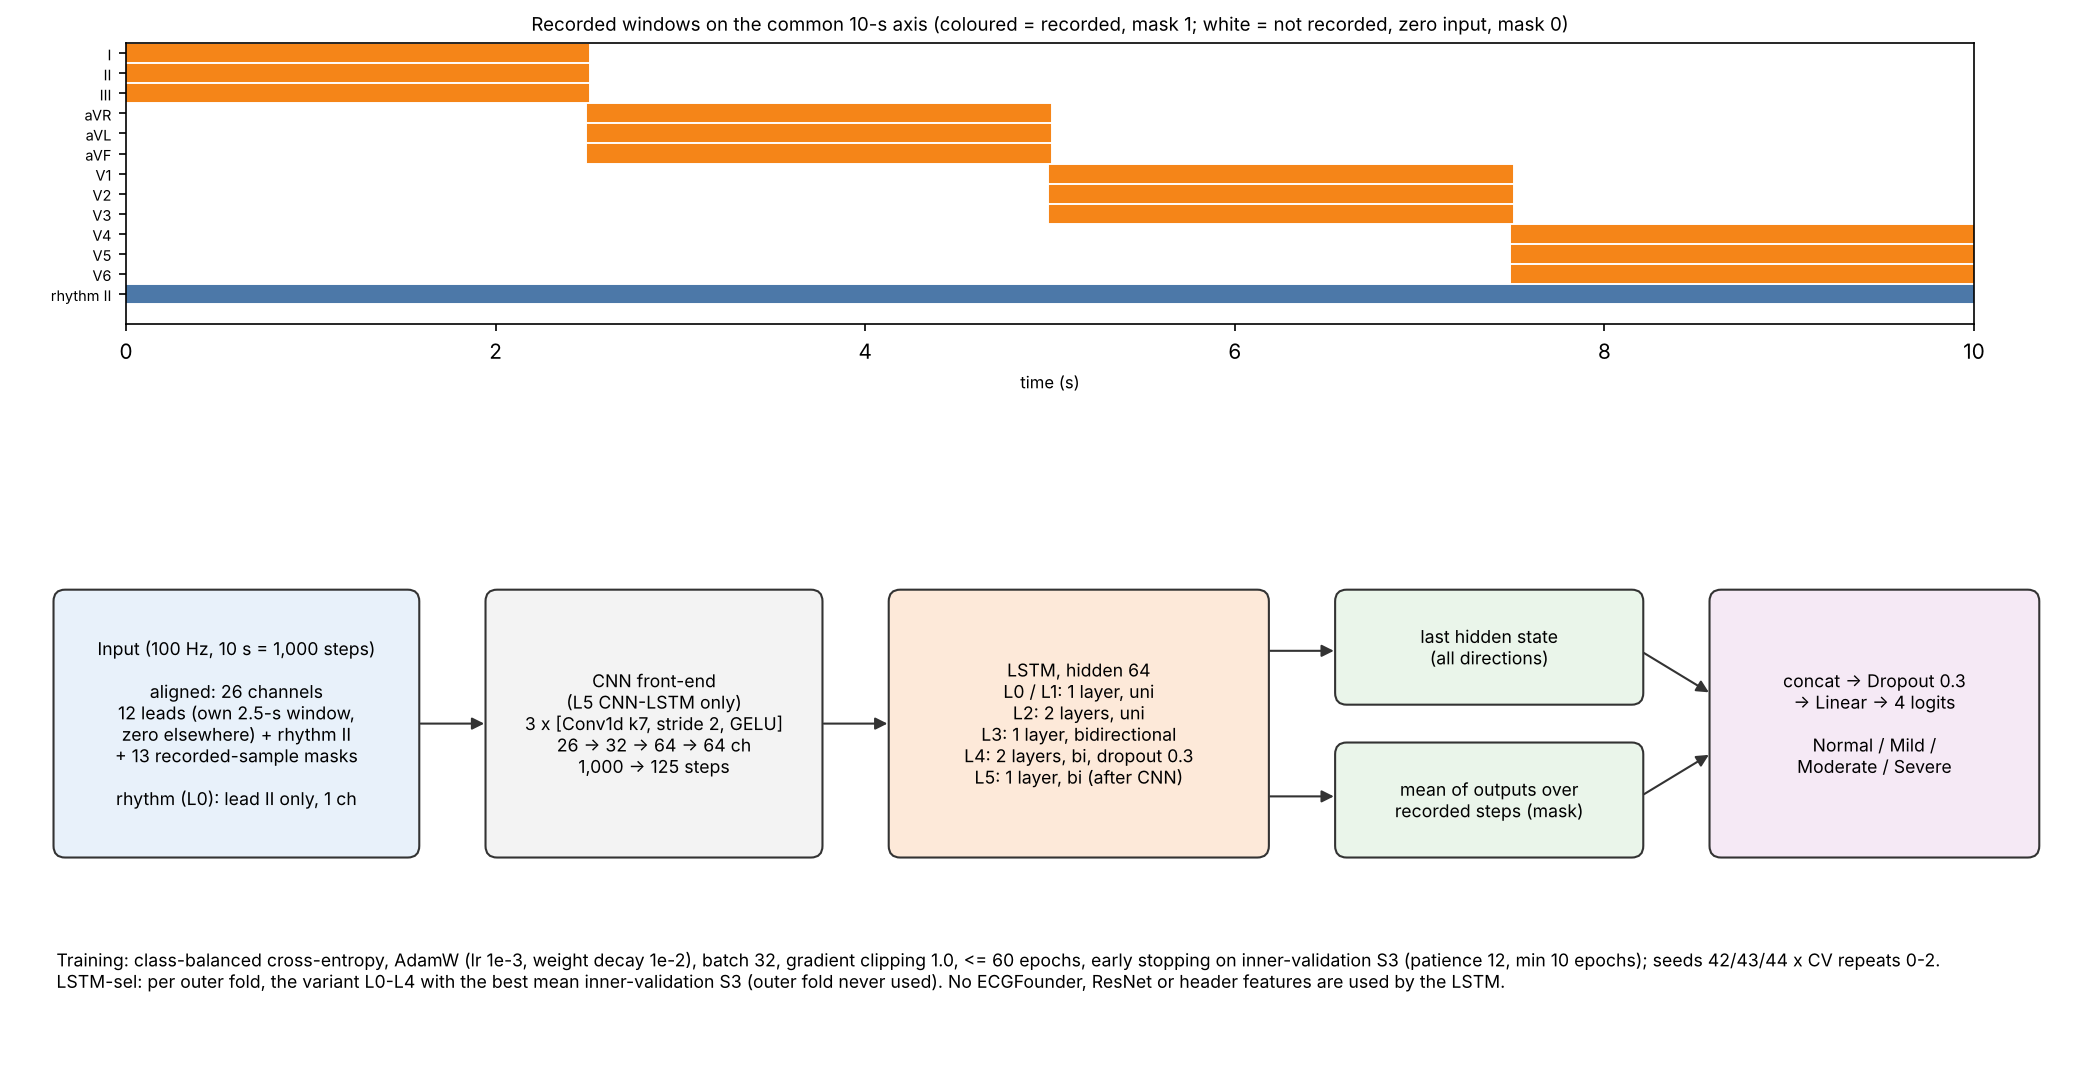
\includegraphics[width=0.95\linewidth]{figures/lstm_architecture.png}
\caption{Top: the printout gives each lead only its own 2.5-s column; only lead II covers 10 s. Bottom: the LSTM /
CNN-LSTM family tested in Phases 6A--6B.}\label{fig:lstm}
\end{figure}

\begin{table}[H]\centering\small
\caption{Phase 6A key results (original labels; corrected 95\,\% CI). ``Adm.'' means every class recall $\ge 0.15$.}\label{tab:p6a}
\begin{adjustbox}{max width=\linewidth}
\begin{tabular}{lccccc}\toprule
Model & Adm. & Accuracy [95\,\% CI] & Macro-F1 & Mild F1 & Mild recall \\\midrule
C3 Phase 5 selected & yes & 0.561 [0.520, 0.603] & 0.448 & 0.221 & 0.177 \\
C1 vote ensemble & yes & 0.547 [0.504, 0.590] & 0.455 & 0.255 & 0.220 \\
C2 calibrated MLP & no & 0.568 [0.534, 0.603] & 0.442 & 0.160 & 0.112 \\
ECGFounder fine-tuned (A1) & yes & 0.536 [0.492, 0.581] & 0.436 & 0.202 & 0.164 \\
ECGFounder frozen, linear & yes & 0.528 [0.484, 0.573] & 0.434 & 0.244 & 0.214 \\
C3 recipe [A270] & yes & 0.561 [0.518, 0.604] & 0.446 & 0.237 & 0.193 \\
C3 recipe [B2] & no & 0.554 [0.511, 0.596] & 0.434 & 0.187 & 0.142 \\
C3 recipe [B3] & no & 0.559 [0.518, 0.600] & 0.426 & 0.144 & 0.103 \\
LSTM L0 (rhythm only) & no & 0.426 [0.387, 0.466] & 0.257 & 0.065 & 0.040 \\
LSTM L2 (best single) & no & 0.483 [0.437, 0.529] & 0.352 & 0.114 & 0.076 \\
LSTM-sel (nested) & no & 0.470 [0.424, 0.515] & 0.344 & 0.122 & 0.081 \\
CNN-LSTM L5 & yes & 0.484 [0.435, 0.532] & 0.368 & 0.219 & 0.191 \\\bottomrule
\end{tabular}
\end{adjustbox}
\end{table}
\textbf{Findings:}
\begin{itemize}
  \item Mild is the main difficulty. Of 185 Mild ECGs, C3 predicts 79 as Normal, 52 as Moderate and 21 as Severe, and
    only 33 as Mild.
  \item A270, B2 and B3 give no improvement (all Holm $p=1.00$). The apparent B2 gain on B2 labels is a
    \emph{definition effect}, not a training effect.
  \item The only significant results are the \emph{inferiority} of the standalone LSTMs (about $-0.09$ accuracy vs C3).
\end{itemize}

% ---------------------------------------------------------------------------------------------------------
\section{Phase 6B: EF thresholds, Normal training size and the LSTM family}\label{sec:p6b}
\textbf{Goal.}
\begin{itemize}
  \item Clinically motivated threshold variants: T50 (Normal $\ge50$\,\%) and T55 (Normal $\ge55$\,\%).
  \item Normal training sizes 300 / 270 / 240 / 200.
  \item Removal of uncertain cases (XUNC).
  \item CNN-LSTM with and without the header, and early or late fusion with ECGFounder.
\end{itemize}
Branch \texttt{research/phase6}, folder \texttt{phase\_6b\_threshold\_sampling\_lstm}.

\begin{table}[H]\centering\small
\caption{Phase 6B: existing recipe under each configuration, scored on the \emph{original} labels (accuracy / Mild recall).}\label{tab:p6b}
\begin{adjustbox}{max width=\linewidth}
\begin{tabular}{lcccc}\toprule
Config & MLP fusion & C1 vote & C3 & LSTM-fixed \\\midrule
ORIG & 0.544 / 0.141 & 0.548 / 0.222 & 0.562 / 0.178 & 0.467 / 0.067 \\
T50 & 0.548 / 0.148 & 0.547 / 0.205 & 0.554 / 0.142 & 0.466 / 0.068 \\
T55 & 0.544 / 0.166 & 0.544 / 0.207 & \textbf{0.569} / 0.186 & 0.459 / 0.097 \\
XUNC & 0.545 / 0.124 & 0.542 / 0.169 & 0.559 / 0.103 & 0.462 / 0.077 \\
N300 & 0.546 / 0.142 & 0.543 / 0.220 & 0.559 / 0.184 & 0.464 / 0.068 \\
N270 & 0.545 / 0.142 & 0.547 / 0.225 & 0.558 / 0.195 & 0.458 / 0.086 \\
N240 & 0.539 / 0.155 & 0.545 / 0.227 & 0.558 / 0.209 & 0.474 / 0.072 \\
N200 & 0.541 / 0.150 & 0.546 / 0.234 & 0.553 / 0.220 & 0.470 / 0.067 \\\bottomrule
\end{tabular}
\end{adjustbox}
\end{table}

\begin{table}[H]\centering\small
\caption{Phase 6B LSTM family and fusions (original labels).}\label{tab:p6b2}
\begin{adjustbox}{max width=\linewidth}
\begin{tabular}{lccccc}\toprule
Model & Accuracy [95\,\% CI] & Macro-F1 & Mild recall & Parameters & Train min/run \\\midrule
F4 vote + LSTM-sel + prior rule & 0.559 [0.517, 0.600] & 0.449 & 0.182 & C1 + 24k--147k & 3.52 \\
F3 vote + LSTM-sel & 0.553 [0.508, 0.597] & 0.453 & 0.198 & C1 + 24k--147k & 2.29 \\
F2 CNN-LSTM + header + f6 & 0.551 [0.517, 0.585] & 0.452 & 0.166 & 198,820 & 0.26 \\
F1 LSTM-fixed + header + f6 & 0.540 [0.507, 0.573] & 0.439 & 0.151 & 130,372 & 0.29 \\
L6 CNN-LSTM + header & 0.497 [0.456, 0.539] & 0.389 & 0.182 & 116,644 & 0.27 \\
L5 CNN-LSTM & 0.484 [0.435, 0.532] & 0.368 & 0.191 & 116,580 & 0.38 \\
LSTM-fixed L3 & 0.467 [0.417, 0.516] & 0.337 & 0.067 & 48,132 & 0.44 \\\bottomrule
\end{tabular}
\end{adjustbox}
\end{table}
\textbf{Findings:}
\begin{itemize}
  \item No configuration or fusion improves on C3; all Holm $p=1.00$. T55 training gives the highest admissible
    figure on original labels (0.569), but $+0.007$ is not significant.
  \item Reducing Normal training ECGs shifts the prior (Mild recall rises, Normal recall falls) without better
    discrimination (Figure~\ref{fig:nsize}).
  \item Under T50 the higher scores are a definition effect: 27 hard borderline Mild ECGs become Normal.
\end{itemize}

\begin{figure}[H]\centering
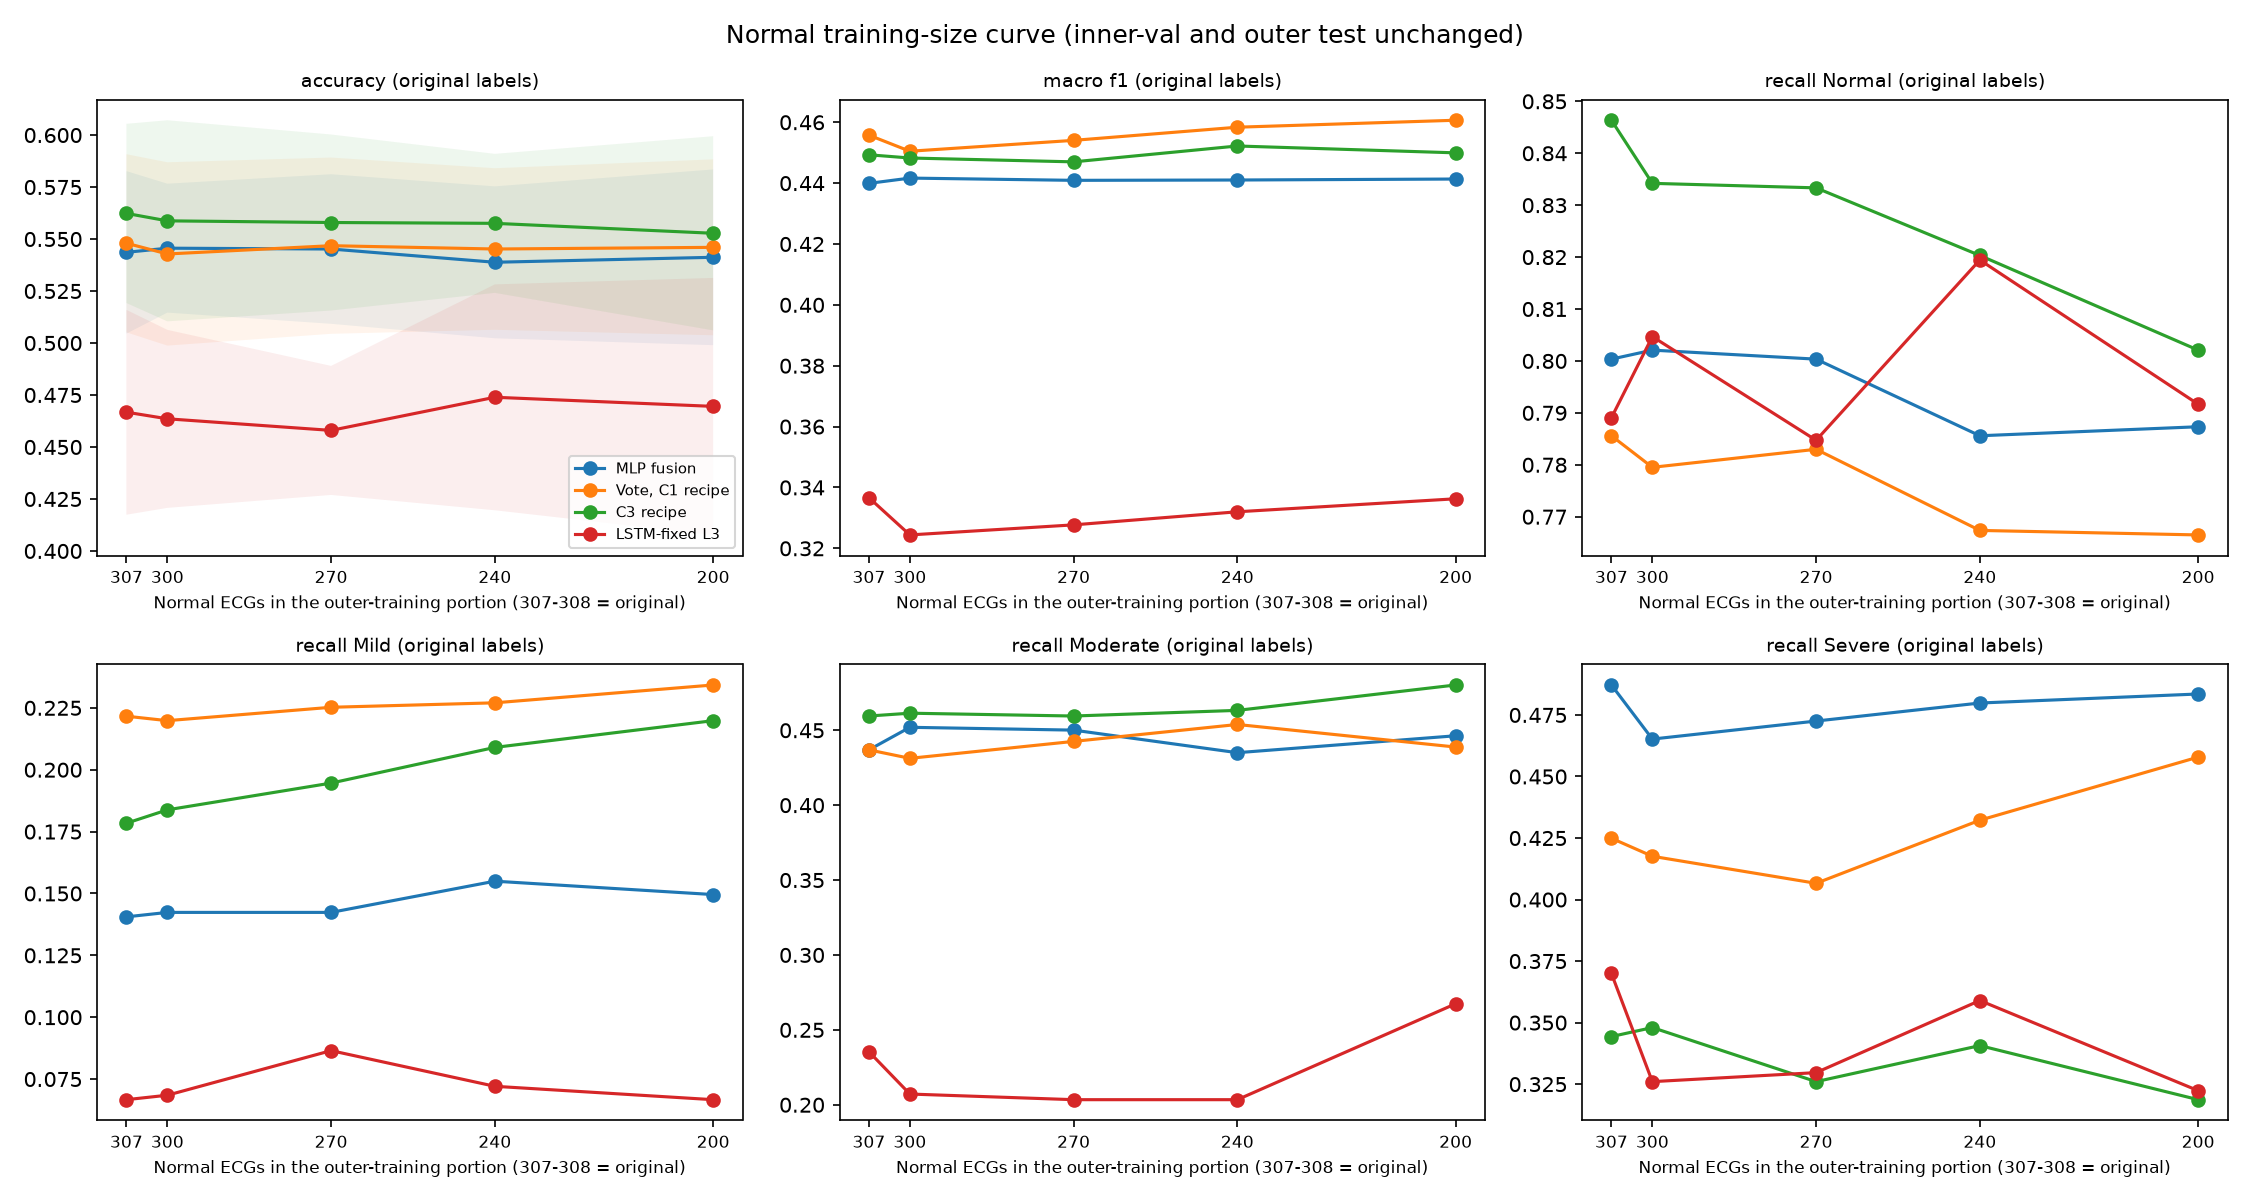
\includegraphics[width=0.7\linewidth]{figures/normal_size_curve.png}
\caption{Normal training size vs accuracy and recall (Phase 6B).}\label{fig:nsize}
\end{figure}

% ---------------------------------------------------------------------------------------------------------
\section{Label-quality and cohort studies (exploratory)}\label{sec:labels}
These studies answered the owner's questions about hard borderline cases, label cleaning and ``reliable'' subsets.
All are on branch \texttt{research/phase6} (\texttt{phase\_6b\_threshold\_sampling\_lstm/}), each with a dated
amendment written before it was run.

\begin{table}[H]\centering\small
\caption{Label / cohort studies. Accuracy on all 837 ECGs unless stated.}\label{tab:labels}
\begin{adjustbox}{max width=\linewidth}
\begin{tabular}{p{4.4cm}p{4.6cm}p{5.4cm}}\toprule
Study & Result & Conclusion \\\midrule
VER: 15 labels corrected to a high-confidence echo & C3 0.565 (+0.004) & label noise explains $<$\,1 point \\
VERB / BRES: resolve or remove borderline cases & gains only by abandoning Mild & not admissible \\
CLEAR: train without border cases & 0.548 all; 0.668 on clear-cut; Mild recall 0.13 & subset gain, not a model gain \\
SUB591: N 200 / Mi 150 / Mo 150 / S all & 0.548 all; 0.489 on subset & no gain \\
HC30: train and test on 395 exact-name, $\le$\,30-day links & 0.594 (C3 trained on all: 0.598) & reliable labels alone do not help \\
HC30F: + all ECG factor families & 0.603 on HC30 (Mild recall 0.25) & $+0.005$, noise level \\
MMCLEAN: remove suspect Mild/Moderate (217) & 0.547 all; 0.677 on kept 620 (Mild recall 0.09) & higher numbers come from easier subsets \\
NF / NFS: noise-free training & 0.546 / 0.552 all; C3 0.707 on 264 clean, clear-cut & cleaning does not raise all-ECG accuracy \\
MILDFIX F1--F3: Mild-aware, ordinal, EF-based rules & 0.537--0.560 & trade accuracy for Mild \\
Circularity check: relabel border cases to model output & 0.764, but random guessing also rises 0.244 $\to$ 0.470 & \textbf{invalid} (circular); excluded \\\bottomrule
\end{tabular}
\end{adjustbox}
\end{table}
\textbf{Selective prediction} (answer only above a nested confidence threshold) first reached about 0.71 on 22\,\% of
ECGs (MMCLEAN, Figure~\ref{fig:coverage}). It was refined in Phase 7 into the final triage model (Section~\ref{sec:final}).

\begin{figure}[H]\centering
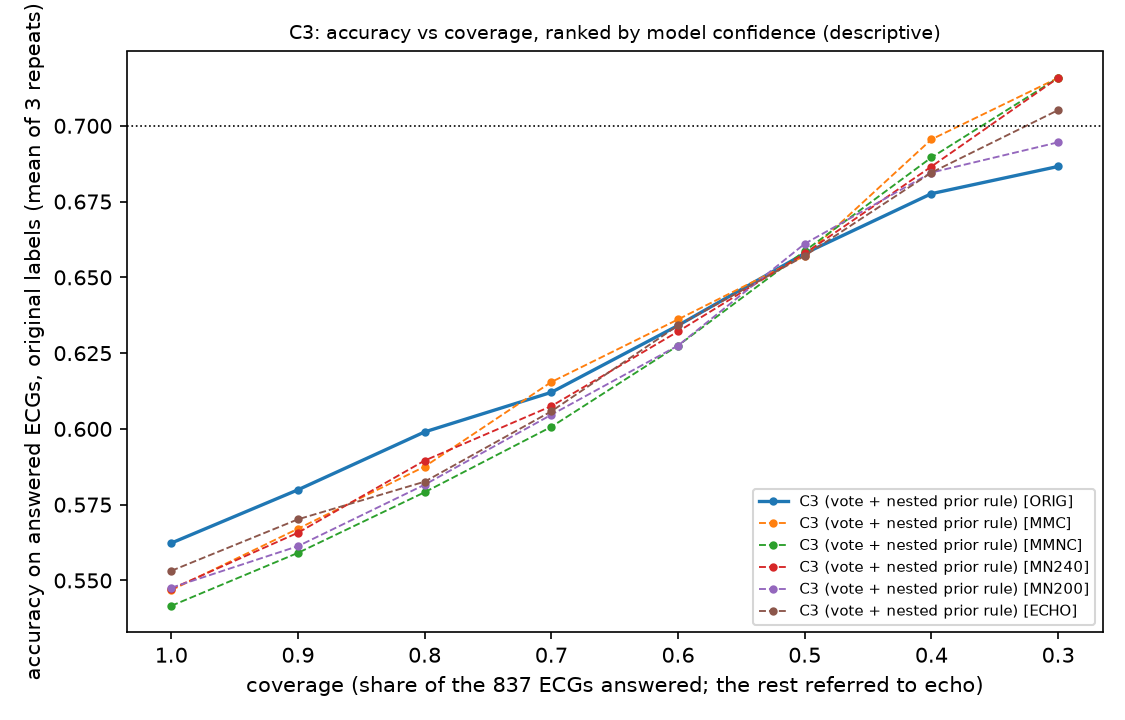
\includegraphics[width=0.62\linewidth]{figures/mmclean_coverage_curve.png}
\caption{Accuracy vs share of ECGs answered (selective prediction).}\label{fig:coverage}
\end{figure}

% ---------------------------------------------------------------------------------------------------------
\section{Phase 7: representation and head experiments, learning curve, triage}\label{sec:p7}
\textbf{Branches:} \texttt{research/phase6} (\texttt{phase\_7/}) and \texttt{research/phase7-testkit} (frozen
model and locked test). \textbf{Pilot gate:} accuracy $\ge +0.010$ or Mild F1 $\ge +0.03$, with macro-F1
$\ge -0.010$. No candidate passed (Table~\ref{tab:p7}).

\begin{table}[H]\centering\small
\caption{Phase 7 pilots (seed 42, 3 repeats).}\label{tab:p7}
\begin{adjustbox}{max width=\linewidth}
\begin{tabular}{llccc}\toprule
Exp. & Candidate & Accuracy & Macro-F1 & Mild P / R / F1 \\\midrule
ref & MLP fusion [header $\|$ f6] & 0.544 & 0.436 & 0.283 / 0.132 / 0.179 \\
E1 & stage-5 mean $\|$ max $\|$ std & 0.517 & 0.409 & 0.263 / 0.146 / 0.187 \\
E1 & per-printed-column stage-5 mean & 0.527 & 0.431 & 0.271 / 0.157 / 0.199 \\
E1 & stage-4 mean $\|$ f6 (multi-scale) & 0.529 & 0.425 & 0.250 / 0.141 / 0.178 \\
E1 & 150 ECGFounder diagnostic outputs & 0.531 & 0.412 & 0.287 / 0.117 / 0.165 \\
E2 & multitask CE + verified-EF regression & 0.545 & 0.440 & 0.289 / 0.142 / 0.191 \\
E2 & boundary-aware soft labels & 0.548 & 0.433 & 0.303 / 0.123 / 0.174 \\
E2 & EF-weighted supervised contrastive & 0.546 & 0.436 & 0.276 / 0.130 / 0.176 \\
E3 & multi-lead 1-D ResNet (repeat 0) & 0.496 & 0.384 & 0.264 / 0.178 / 0.213 \\
E3 & 1-D ResNet + header (repeat 0) & 0.485 & 0.378 & 0.243 / 0.189 / 0.213 \\\bottomrule
\end{tabular}
\end{adjustbox}
\end{table}

\paragraph{E5: learning curve} (Figure~\ref{fig:lc}):
\begin{itemize}
  \item each doubling of training data gives $+1.4$ accuracy points, with no trend in Mild F1;
  \item the EF error SD falls by 0.44 points per doubling (0.66 on verified-EF ECGs);
  \item extrapolation: about $10^5$ ECGs of current label quality would give about 0.65.
\end{itemize}

\begin{figure}[H]\centering
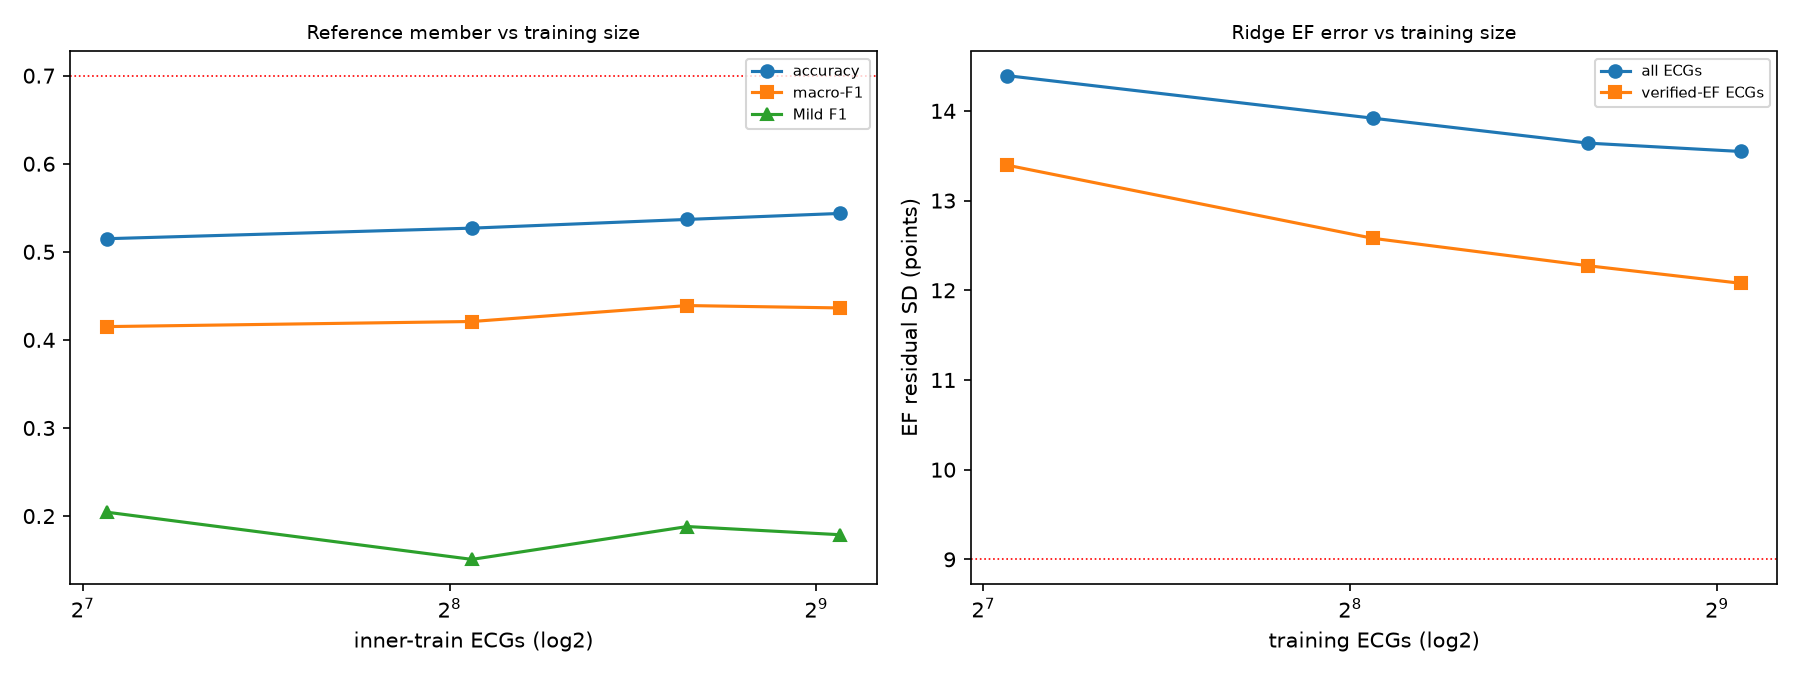
\includegraphics[width=0.95\linewidth]{figures/phase7_learning_curve.png}
\caption{Phase 7 learning curve: classification metrics (left) and EF error (right) vs training size.}\label{fig:lc}
\end{figure}

\paragraph{E6: header-free cascades.}
\begin{itemize}
  \item EF-grading stage 1 alone: 0.693 on 53\,\% answered (G2T-img); 0.694 on 56\,\% when it must agree with IMG-C3
    (AGT-img, the final triage).
  \item As complete four-class classifiers the cascades reach 0.548--0.568, no genuine gain.
  \item Stage 1 answers almost only Normal.
\end{itemize}

\paragraph{E7: Mild-aware selective prediction.}
\begin{itemize}
  \item Accuracy $\ge 0.70$ together with detecting $\ge 10$\,\% of Mild patients is \emph{infeasible} in all 15
    training folds.
  \item Even the most confident Mild calls are right only 20--50\,\% of the time.
\end{itemize}

% ---------------------------------------------------------------------------------------------------------
\section{Final push on image-only four-class accuracy}\label{sec:push}
At the owner's request (image only, Mild $\ge 15$\,\%), four further pre-registered studies were run. They are on
branch \texttt{research/phase6}: \texttt{HIER\_REPORT.md}, \texttt{ENH\_REPORT.md}, \texttt{ULT\_REPORT.md} and
\texttt{ECHONEXT\_REPORT.md}.

\begin{table}[H]\centering\small
\caption{Image-only four-class models, all 837 ECGs (no header, age or sex input).}\label{tab:push}
\begin{adjustbox}{max width=\linewidth}
\begin{tabular}{p{6.2cm}cc}\toprule
Model & Accuracy [95\,\% CI] & Recall N / Mi / Mo / S \\\midrule
HIER: two-stage (N / middle / S, then Mi vs Mo) & 0.558 [0.522, 0.594] & 0.86 / 0.17 / 0.41 / 0.34 \\
HIER-ext (wider tuning grid) & 0.570 [0.527, 0.612] & 0.88 / 0.16 / 0.43 / 0.34 \\
ENH: synth 10-s reconstruction $\to$ ECGFounder (M2) & 0.528 & 0.76 / 0.18 / 0.44 / 0.41 \\
ENH: same head on aligned input (D1 reference) & 0.537 & 0.78 / 0.21 / 0.41 / 0.42 \\
ENH: median-beat shape (M3) & 0.467 & 0.68 / 0.19 / 0.36 / 0.33 \\
ENH: MiniRocket (M4) & 0.504 & 0.74 / 0.22 / 0.38 / 0.33 \\
ENH: EF-ordinal ridge (M6) & 0.534 & 0.95 / 0.29 / 0.00 / 0.29 \\
ENH-vote (6 members, tuned class weights) & 0.569 [0.527, 0.610] & 0.88 / 0.17 / 0.46 / 0.29 \\
\textbf{ULT-stack (10 members + predicted EF)} & \textbf{0.571 [0.542, 0.600]} & 0.91 / 0.16 / 0.42 / 0.29 \\
ULT2-stack (+ EchoNext-Mini external model) & 0.569 [0.538, 0.599] & 0.90 / 0.15 / 0.44 / 0.28 \\
EchoNext-Mini outputs + LR alone & 0.486 [0.436, 0.536] & 0.72 / 0.11 / 0.36 / 0.53 \\\bottomrule
\end{tabular}
\end{adjustbox}
\end{table}
\textbf{Findings:}
\begin{itemize}
  \item \textbf{Two-stage:} stage 1 (Normal / middle / Severe) is right 66--67\,\% of the time. Stage 2 (Mild vs
    Moderate) is right only 53--58\,\%, close to a coin flip.
  \item \textbf{Reconstruction:} a faithful beat-synchronous 10-s 12-lead reconstruction (template $r=0.98$) adds
    no EF information.
  \item \textbf{External knowledge:} EchoNext-Mini (Hughes et al., 2026; Poterucha et al., 2025), trained on about
    100,000 US patients, transfers to the printouts (AUROC 0.79 for EF $\le 45$\,\%). It is weaker than the in-house
    EF model (0.86) and adds no accuracy.
  \item \textbf{Ensembles:} all ensembles plateau at $0.57\pm0.01$ (Figure~\ref{fig:landscape}).
\end{itemize}

% ---------------------------------------------------------------------------------------------------------
\section{Sensitivity to the class definition (band sweep)}\label{sec:bands}
\begin{itemize}
  \item \textbf{Sweep:} 3,313 definitions (Normal limit 45--56, Mild/Moderate 35--46, Moderate/Severe 25--36, sex
    offset 0/2) were evaluated with one header-free EF model. 1,457 of them are feasible (every class $\ge 60$
    ECGs, both middle bands $\ge 5$ points wide).
  \item \textbf{Confirmation:} the selected definitions were retrained.
  \item \textbf{Result:} the clinically pre-specified \textbf{ESC 2021} definition (Normal $\ge 50$, Mild 41--49,
    Moderate 30--40, Severe $<30$) gives \textbf{0.626 [0.588, 0.664]} with every class detected (Mild 17\,\%,
    Moderate 42\,\%).
  \item \textbf{Trade-off:} no definition detects both Mild and Moderate well (Figure~\ref{fig:bands}).
\end{itemize}
These figures belong to a different task definition and are reported only as a sensitivity analysis.

\begin{table}[H]\centering\small
\caption{Confirmed band definitions (retrained header-free vote).}\label{tab:bands}
\begin{adjustbox}{max width=\linewidth}
\begin{tabular}{lcccc}\toprule
Definition & N / Mi / Mo / S ECGs & Accuracy [95\,\% CI] & $\kappa$ & Detected N / Mi / Mo / S \\\midrule
Original limits on echo EF & 415 / 170 / 165 / 87 & 0.594 [0.560, 0.627] & 0.353 & 91 / 20 / 32 / 38\,\% \\
\textbf{ESC 2021} & 446 / 139 / 176 / 76 & \textbf{0.626} [0.588, 0.664] & 0.384 & 90 / 17 / 42 / 35\,\% \\
Best Mild detection ($>$51 / 38 / 31) & 439 / 197 / 114 / 87 & 0.619 [0.593, 0.645] & 0.380 & 90 / 28 / 25 / 43\,\% \\
Best $\kappa$ ($>$52 / 46 / 29) & 428 / 70 / 272 / 67 & 0.634 [0.591, 0.678] & 0.399 & 87 / 12 / 49 / 27\,\% \\\bottomrule
\end{tabular}
\end{adjustbox}
\end{table}

\begin{figure}[H]\centering
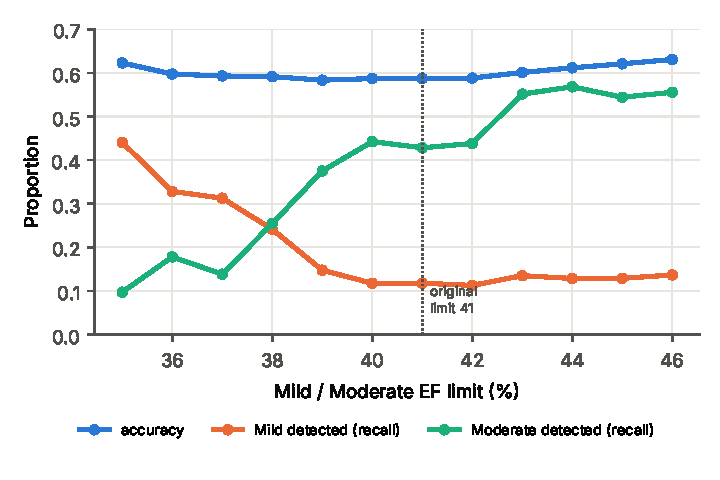
\includegraphics[width=0.62\linewidth]{figures/fig_band_sweep.pdf}
\caption{Moving the Mild/Moderate limit trades Mild detection against Moderate detection.}\label{fig:bands}
\end{figure}
